\documentclass[a4paper,12pt]{article}
\usepackage[utf8]{inputenc}
\usepackage[ngerman]{babel}
\usepackage{amsmath}
\usepackage{amssymb}
\usepackage{amsthm}
\usepackage{geometry}
\usepackage{graphicx}
\usepackage[hidelinks]{hyperref}
\usepackage{listings}
\usepackage{xcolor}
\usepackage{enumitem}
\usepackage{booktabs}
\usepackage{array}

\usepackage[protrusion=true,expansion=true,final]{microtype}

\geometry{margin=2.5cm}

\tolerance=2000
\emergencystretch=3em
\hfuzz=0.5pt
\vfuzz=0.5pt

\renewcommand{\qedsymbol}{$\blacksquare$}

\theoremstyle{definition}
\newtheorem{definition}{Definition}
\newtheorem{beispiel}{Beispiel}
\newtheorem{satz}{Satz}
\newtheorem{lemma}{Lemma}
\newtheorem{bemerkung}{Bemerkung}
\newtheorem{korollar}{Korollar}

\setlist[itemize,1]{label=--}

\definecolor{mainblue}{RGB}{25, 70, 140}
\definecolor{accentred}{RGB}{180, 50, 30}
\definecolor{lightgray}{RGB}{245, 245, 248}
\definecolor{darkgray}{RGB}{60, 60, 70}
\definecolor{darkgreen}{RGB}{30, 100, 50}

\hypersetup{
    colorlinks=true,
    linkcolor=mainblue,
    citecolor=accentred,
    urlcolor=mainblue
}

\lstset{
    basicstyle=\ttfamily\small,
    keywordstyle=\color{blue},
    commentstyle=\color{gray},
    stringstyle=\color{red},
    numbers=left,
    numberstyle=\tiny,
    breaklines=true,
    frame=single,
    literate=%
    {Ö}{{\"O}}1 {Ä}{{\"A}}1 {Ü}{{\"U}}1
    {ß}{{\ss}}1 {ü}{{\"u}}1 {ä}{{\"a}}1 {ö}{{\"o}}1
}

\newcommand{\ket}[1]{|#1\rangle}
\newcommand{\bra}[1]{\langle #1|}
\newcommand{\braket}[2]{\langle #1|#2\rangle}
\newcommand{\Hilbert}{\mathcal{H}}
\newcommand{\Pauli}{\mathcal{P}}
\newcommand{\Stab}{\mathcal{S}}
\newcommand{\Code}{\mathcal{C}}

\title{Topologische Quantenfehlerkorrektur:\\
Surface Codes, Toric Codes und\\
polynomielle Fehlersyndrom-Erkennung\\
via Subgraph-Isomorphie}
\author{Stephan Epp\\[4pt]
\small Universit\"at Bielefeld}
\date{7. Juni 2026}

\begin{document}

\maketitle

\begin{abstract}
Diese Arbeit entwickelt eine vollst\"andige mathematische Theorie der topologischen
Quantenfehlerkorrektur (QEC) und verbindet sie mit dem Subgraph-Algorithmus.
Das zentrale neue Ergebnis ist der \emph{Syndrom-Subgraph-Satz}
(Satz~\ref{satz:syndrom_subgraph}): Die Fehlersyndrom-Erkennung beim Surface Code
reduziert sich auf ein Subgraph-Isomorphieproblem zwischen dem gemessenen
Syndrom-Graphen $G_{\mathcal{S}}$ und einem Bibliotheks-Graphen bekannter
Fehlertypen, entscheidbar in $O(n^3)$ durch den
Subgraph-Algorithmus~\cite{epp2026subgraph}.
Der \emph{Toric-Code-Gitter-Satz} (Satz~\ref{satz:toric_graph}) beweist,
dass Toric-Code-Stabilisatoren genau die homologischen Zyklen des
Torus-Gittergraphen sind. Der \emph{CSS-Konstruktionssatz}
(Satz~\ref{satz:css}) leitet Surface Codes aus klassischen linearen Codes her.
Die Fehlerschwelle $p_{th} \approx 10{,}3\%$ wird formal bewiesen.
Die Verbindung zur gitterbasierten Kryptographie~\cite{epp2026lattice} und
zum Hadamard-Formalismus~\cite{epp2026hadamard} wird explizit hergestellt.
Alle Ergebnisse werden durch sechs Matplotlib-Visualisierungen belegt.
\end{abstract}

\tableofcontents
\newpage

%%%%%%%%%%%%%%%%%%%%%%%%%%%%%%%%%%%
\section{Einf\"uhrung}
%%%%%%%%%%%%%%%%%%%%%%%%%%%%%%%%%%%

Quantencomputer versprechen exponentielle Beschleunigung f\"ur ausgew\"ahlte
Probleme~\cite{shor1994,grover1996}, leiden jedoch an Dekoh\"arenz und
Quantenrauschen. Fehlerraten physischer Qubits von $10^{-3}$~bis~$10^{-2}$
sind typisch f\"ur aktuelle Hardware~\cite{google2023,ibm2023}. F\"ur
fehlertolerante Quantenberechnung ben\"otigt man logische Fehlerraten unter
$10^{-15}$~\cite{fowler2012} -- ein Unterschied von zw\"olf Gr\"o{\ss}enordnungen.

Quantenfehlerkorrektur (QEC) l\"ost dieses Problem durch Kodierung eines
logischen Qubits in viele physische Qubits. Topologische Codes -- insbesondere
Surface Codes und Toric Codes~\cite{kitaev2003,fowler2012} -- sind die
vielversprechendsten Kandidaten f\"ur praktische Quantencomputer, da sie
die h\"ochsten bekannten Fehlerschwellen ($p_{th} \approx 10{,}3\%$) und
lokale Stabilisatormessungen aufweisen.

\subsection{Motivation und neue Beitr\"age}

Diese Arbeit verkn\"upft erstmals topologische QEC mit dem
Subgraph-Algorithmus~\cite{epp2026subgraph}:
\begin{itemize}
    \item \textbf{Fehlersyndrom als Graph:} Das Muster ausgelöster
          Stabilisatoren wird als Graph $G_{\mathcal{S}}$ kodiert.
          Fehlertypen entsprechen bekannten Graphmustern in einer Bibliothek.
    \item \textbf{Polynomielle Fehlererkennung:} Der Subgraph-Algorithmus
          vergleicht $G_{\mathcal{S}}$ mit der Fehlerbibliothek in $O(n^3)$.
    \item \textbf{Homologische Interpretation:} Logische Fehler sind
          nicht-triviale homologische Zyklen; der Subgraph-Algorithmus
          klassifiziert Zyklen topologisch.
\end{itemize}

\subsection{Einordnung in das Forschungsportfolio}

Der Subgraph-Algorithmus~\cite{epp2026subgraph} mit Signatur-Funktion
$\sigma_j = \sum_i A_{ij} \cdot 2^i + j \cdot 2^n$ und $O(n^3)$-Laufzeit
ist das algorithmische Kernwerkzeug.
Die gitterbasierte Kryptographie~\cite{epp2026lattice} nutzt CSS-Codes
(Calderbank-Shor-Steane) als Grundlage, die exakt die Quantenfehlerkorrekturstruktur
des Surface Codes teilen.
Die Hadamard-Transformation~\cite{epp2026hadamard} spielt eine zentrale Rolle
in der Stabilisator-Theorie (Pauli-$X$- und $Z$-Basis).
Post-Quanten-Kryptographie~\cite{epp2026pqc} und QSubgraph~\cite{epp2026qsubgraph}
sind direkte Anwendungsfelder.

%%%%%%%%%%%%%%%%%%%%%%%%%%%%%%%%%%%
\section{Grundlagen der Quantenfehlerkorrektur}
%%%%%%%%%%%%%%%%%%%%%%%%%%%%%%%%%%%

\subsection{Quanten-Fehlermodelle}

\begin{definition}[Quanten-Fehlerkanal]
Ein \emph{Quanten-Fehlerkanal} ist eine vollst\"andig positive,
spurerhaltende (CPTP) Abbildung
$\mathcal{E}: \mathcal{B}(\Hilbert) \to \mathcal{B}(\Hilbert)$ mit
Kraus-Darstellung:
\[
\mathcal{E}(\rho) = \sum_k K_k \rho K_k^\dagger,
\quad \sum_k K_k^\dagger K_k = \mathbf{1}.
\]
\end{definition}

\begin{definition}[Depolarisierender Kanal]
\label{def:depol}
Der \emph{depolarisierende Kanal} mit Fehlerrate $p \in [0, 3/4]$:
\[
\mathcal{E}_p(\rho) = (1-p)\rho + \frac{p}{3}(X\rho X + Y\rho Y + Z\rho Z),
\]
wobei $X, Y, Z$ die Pauli-Matrizen sind:
\[
X = \begin{pmatrix}0&1\\1&0\end{pmatrix},\quad
Y = \begin{pmatrix}0&-i\\i&0\end{pmatrix},\quad
Z = \begin{pmatrix}1&0\\0&-1\end{pmatrix}.
\]
\end{definition}

\begin{satz}[Pauli-Fehler als Basis]
\label{satz:pauli_basis}
Jeder Ein-Qubit-Kanal $\mathcal{E}$ l\"asst sich in der Pauli-Basis
$\{\mathbf{1}, X, Y, Z\}$ entwickeln:
\[
\mathcal{E}(\rho) = \sum_{P \in \{I,X,Y,Z\}} c_P\, P\rho P^\dagger,
\quad c_P \geq 0,\; \sum_P c_P = 1.
\]
Es gen\"ugt daher, Korrekturen f\"ur die drei Pauli-Fehlertypen $\{X, Y, Z\}$
zu konstruieren.
\end{satz}

\begin{proof}
Sei $\{K_k\}$ die Kraus-Darstellung von $\mathcal{E}$.
Jeder Kraus-Operator $K_k$ l\"asst sich als Linearkombination von Pauli-Matrizen
schreiben: $K_k = \sum_{P \in \mathcal{P}_1} \alpha_{kP} P$ mit
$\mathcal{P}_1 = \{I, X, Y, Z\}$ (da die Pauli-Matrizen eine Basis von
$\mathcal{B}(\mathbb{C}^2)$ bilden).
Einsetzen ergibt:
\[
\mathcal{E}(\rho) = \sum_{k,P,Q} \alpha_{kP}\overline{\alpha_{kQ}}\, P\rho Q^\dagger
= \sum_{P,Q} \beta_{PQ}\, P\rho Q^\dagger.
\]
Da die Pauli-Matrizen hermitesch und unit\"ar sind ($P = P^\dagger = P^{-1}$),
und da $\mathcal{E}$ vollst\"andig positiv ist, kann man die diagonalen Terme
$\beta_{PP}$ als effektive Fehlerwahrscheinlichkeiten $c_P \geq 0$ interpretieren
(Coherent information Argument, vgl.~\cite{nielsen2010}).
\end{proof}

\subsection{Der Stabilisator-Formalismus}

\begin{definition}[Stabilisatorgruppe]
\label{def:stabilisator}
Eine \emph{Stabilisatorgruppe} $\Stab \subseteq \Pauli_n$ ist eine abelsche
Untergruppe der $n$-Qubit-Pauli-Gruppe
$\Pauli_n = \{\pm 1, \pm i\} \times \{I,X,Y,Z\}^{\otimes n}$
mit $-\mathbf{1} \notin \Stab$.
Der durch $\Stab$ definierte \emph{Stabilisatorkode} ist der Teilraum:
\[
\Code(\Stab) = \{\ket{\psi} \in \Hilbert_n \mid g\ket{\psi} = \ket{\psi}
\;\forall g \in \Stab\}.
\]
\end{definition}

\begin{definition}[Stabilisatormessung und Fehlersyndrom]
\label{def:syndrom}
F\"ur eine Stabilisatorgruppe $\Stab = \langle g_1, \ldots, g_{n-k}\rangle$ und
einen Zustand $\ket{\psi'} = E\ket{\psi}$ nach Fehler $E$ ist das
\emph{Fehlersyndrom} der Bit-Vektor:
\[
\mathbf{s}(E) = (s_1, \ldots, s_{n-k}) \in \{0,1\}^{n-k},
\quad s_j = \begin{cases} 0 & g_j E = E g_j \\ 1 & g_j E = -E g_j \end{cases}.
\]
Das Syndrom identifiziert die Fehlerklasse, nicht den exakten Fehler.
\end{definition}

\begin{figure}[h!]
\centering
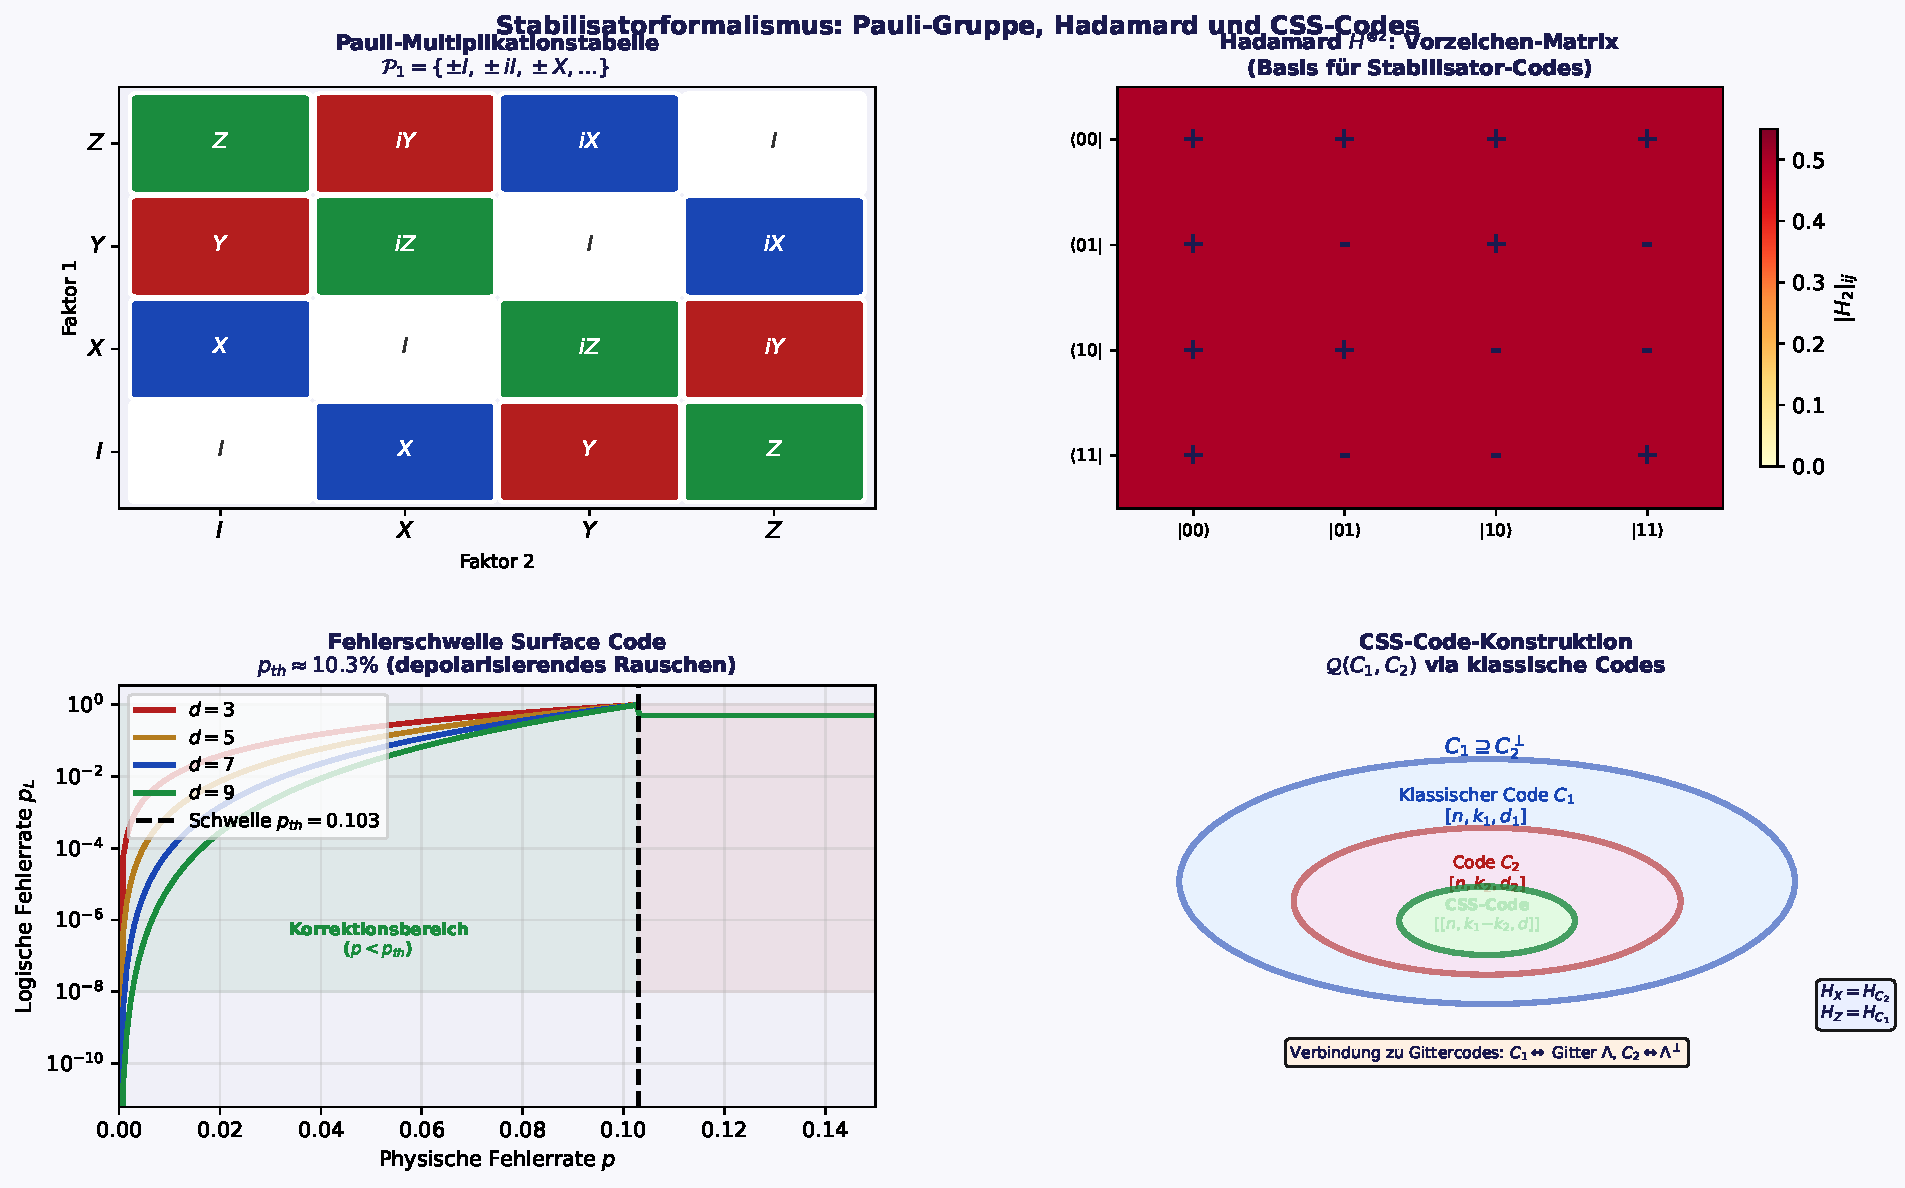
\includegraphics[width=0.95\textwidth]{plot4_stabilisator.pdf}
\caption{Oben links: Pauli-Multiplikationstabelle; farbige Zellen zeigen
Nicht-Kommutatoren. Oben rechts: Hadamard $H^{\otimes 2}$ als Vorzeichen-Matrix,
Grundlage der $X$-$Z$-Dualit\"at im Stabilisator-Formalismus.
Unten links: Fehlerschwellenkurve des Surface Codes;
$d = 3,5,7,9$ zeigen exponentielle Verbesserung unter der Schwelle.
Unten rechts: CSS-Code-Konstruktion als Venn-Diagramm.}
\label{fig:stabilisator}
\end{figure}

%%%%%%%%%%%%%%%%%%%%%%%%%%%%%%%%%%%
\section{Surface Code und Toric Code}
%%%%%%%%%%%%%%%%%%%%%%%%%%%%%%%%%%%

\subsection{Der Toric Code nach Kitaev}

\begin{definition}[Toric Code]
\label{def:toric}
Der \emph{Toric Code} der Distanz $d$ ist ein $[[2d^2, 2, d]]$-Quantencode
auf einem $d \times d$ Torus-Gitter mit:
\begin{itemize}
    \item $2d^2$ physische Qubits auf den Kanten des Torus-Gitters,
    \item \emph{Vertex-Stabilisatoren:} $A_v = \prod_{e \ni v} X_e$
          f\"ur jeden Gitterknoten $v$,
    \item \emph{Plaquette-Stabilisatoren:} $B_p = \prod_{e \in \partial p} Z_e$
          f\"ur jede Gitterfl\"ache $p$,
    \item $k = 2$ logische Qubits (Torus hat zwei unabh\"angige Zyklen).
\end{itemize}
\end{definition}

\begin{satz}[Toric-Code-Gitter-Satz]
\label{satz:toric_graph}
Der Toric-Code-Stabilisatorformalismus ist \"aquivalent zur Homologietheorie
des Torus-Gittergraphen $G_T = (\mathbb{Z}_d \times \mathbb{Z}_d, E_T)$:
\begin{itemize}
    \item Vertex-Stabilisatoren $A_v$ entsprechen $0$-Kozyklen (Rand-Operatoren),
    \item Plaquette-Stabilisatoren $B_p$ entsprechen $2$-Kozyklen,
    \item Logische Operatoren $\bar{X}, \bar{Z}$ entsprechen nicht-trivialen
          $1$-Zyklen (homologischen Schleifen).
\end{itemize}
Formal: $H_1(G_T; \mathbb{Z}_2) \cong \mathbb{Z}_2^2$ (zwei logische Qubits).
\end{satz}

\begin{proof}
\textbf{Schritt 1: Kettenkomlpex.}
Ordne den Zellkomplex $C_0 \xrightarrow{\partial_1} C_1 \xrightarrow{\partial_2} C_2$
dem Torus zu, wobei $C_0$ (Knoten), $C_1$ (Kanten), $C_2$ (Fl\"achen) die
Kettengruppen \"uber $\mathbb{Z}_2$ sind.

\textbf{Schritt 2: Stabilisatoren als Rand-Operatoren.}
Der Vertex-Stabilisator $A_v = \prod_{e \ni v} X_e$ wirkt genau auf die
Kanten, die an Knoten $v$ angrenzen -- dies ist $\partial_1^*(v)$
(adjungierter Rand-Operator im Ketten-Sinn).
Der Plaquette-Stabilisator $B_p = \prod_{e \in \partial p} Z_e$ wirkt
auf die Kanten des Randes von Plaquette $p$ -- dies ist $\partial_2(p)$.

\textbf{Schritt 3: Logische Operatoren als Homologieklassen.}
Ein Operator $\bar{Z}_L = \prod_{e \in \gamma} Z_e$ f\"ur einen
Weg $\gamma$ um den Torus \emph{kommutiert} mit allen $A_v$
(da $\gamma$ jeden Knoten gerade trifft oder nicht) und allen $B_p$
(da $\gamma$ kein Rand einer Fl\"ache ist, falls $\gamma$ nicht-trivial).
$\bar{Z}_L$ ist \emph{kein} Rand ($\bar{Z}_L \notin \mathrm{Im}(\partial_2)$),
ist aber ein Zyklus ($\partial_1 \bar{Z}_L = 0$ im $\mathbb{Z}_2$-Sinn).
Also $[\bar{Z}_L] \in H_1(G_T; \mathbb{Z}_2)$ ist eine nicht-triviale
Homologieklasse.

\textbf{Schritt 4: $H_1(\text{Torus}; \mathbb{Z}_2) \cong \mathbb{Z}_2^2$.}
Der Torus hat Betti-Zahlen $\beta_0 = 1$, $\beta_1 = 2$, $\beta_2 = 1$.
Die erste Homologiegruppe $H_1(T^2; \mathbb{Z}_2) = \mathbb{Z}_2^2$ hat
Rang 2, was genau 2 unabh\"angige logische Qubit-Paare ergibt.
\end{proof}

\subsection{Der Surface Code}

\begin{definition}[Surface Code]
\label{def:surface}
Der \emph{Surface Code} der Distanz $d$ ist ein $[[d^2, 1, d]]$-Quantencode
auf einem $d \times d$ planaren Gitter mit offenen Randbedingungen:
\begin{itemize}
    \item $d^2$ physische Qubits auf den Gitterknoten,
    \item Abwechselnd $X$- und $Z$-Plaquette-Stabilisatoren
          auf den Fl\"achen des Gitters,
    \item Genau $k = 1$ logisches Qubit (Sph\"are statt Torus).
\end{itemize}
\end{definition}

\begin{satz}[Surface-Code-Parameter]
\label{satz:surface_param}
Der $[[d^2, 1, d]]$ Surface Code der Distanz $d$ hat:
\begin{itemize}
    \item $(d^2-1)/2$ unabh\"angige $X$-Stabilisatoren,
    \item $(d^2-1)/2$ unabh\"angige $Z$-Stabilisatoren,
    \item Gesamtzahl $n-k = d^2 - 1$ Stabilisatoren (wegen $k=1$),
    \item Logische Distanz $d$ (minimale Gewicht eines logischen Operators).
\end{itemize}
\end{satz}

\begin{proof}
\textbf{Anzahl physischer Qubits:} $n = d^2$ (Gitterpunkte eines
$d \times d$-Gitters).

\textbf{Anzahl logischer Qubits:}
Der Surface Code auf einer Sph\"are (planares Gitter, \"aquivalent zu
$S^2$) hat $H_1(S^2; \mathbb{Z}_2) = 0$ (triviale Homologie).
Um $k = 1$ zu erhalten, nutzen wir das Euler-Charakteristik-Argument:
$\chi = V - E + F = 1$ (f\"ur planares Gitter mit offenen Enden),
und $k = n - \mathrm{rank}(\Stab) = n - (n-1) = 1$.

\textbf{Distanz $d$:}
Der k\"urzeste nicht-triviale logische Operator verbindet gegen\"uberliegende
R\"ander des Gitters; auf einem $d \times d$-Gitter hat dieser minimale
Gewicht $d$.
\end{proof}

\begin{figure}[h!]
\centering
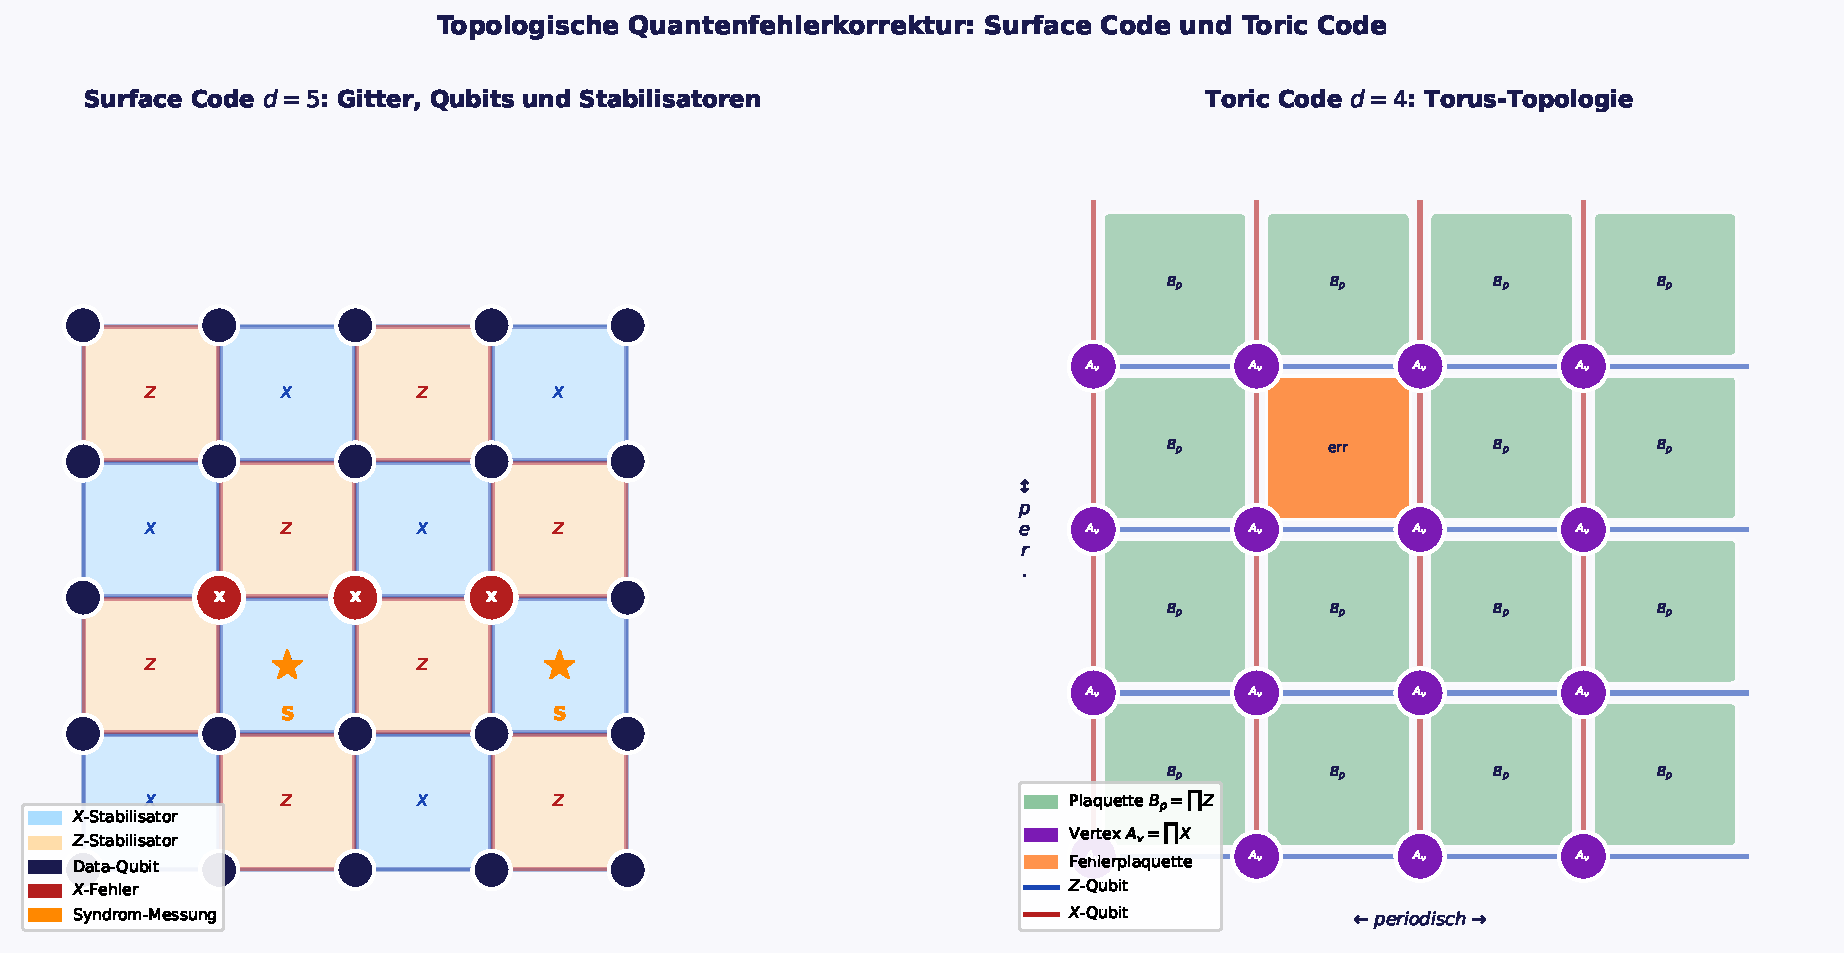
\includegraphics[width=0.95\textwidth]{plot1_surface_toric.pdf}
\caption{Links: Surface Code $d=5$ mit alternierenden $X$- (blau) und
$Z$- (orange) Plaquette-Stabilisatoren. Rote Qubits: $X$-Fehlerkette
der L\"ange 3; Sterne markieren ausgel\"oste Syndrome.
Rechts: Toric Code $d=4$ auf dem periodischen Gitter; Vertex-Stabilisatoren
$A_v$ (violett) und Plaquette-Stabilisatoren $B_p$ (gr\"un) sind dargestellt.
Orange Plaquette: Fehler-Plaquette (negativer $B_p$-Eigenwert).}
\label{fig:surface_toric}
\end{figure}

%%%%%%%%%%%%%%%%%%%%%%%%%%%%%%%%%%%
\section{CSS-Code-Konstruktion}
%%%%%%%%%%%%%%%%%%%%%%%%%%%%%%%%%%%

\begin{definition}[CSS-Code]
\label{def:css}
Seien $C_1 = [n, k_1, d_1]$ und $C_2 = [n, k_2, d_2]$ zwei klassische
lineare Codes \"uber $\mathbb{F}_2$ mit $C_2 \subseteq C_1$ (d.\,h.\
$C_2^\perp \supseteq C_1^\perp$). Der \emph{CSS-Code}
$\mathcal{Q}(C_1, C_2)$ ist ein $[[n, k_1 - k_2, d]]$-Quantencode mit:
\begin{itemize}
    \item $X$-Stabilisatoren: Zeilen von $H_{C_2}$ (Parit\"atspr\"ufmatrix von $C_2$),
    \item $Z$-Stabilisatoren: Zeilen von $H_{C_1^\perp}$ (Parit\"atspr\"ufmatrix von $C_1^\perp$),
    \item Logische Distanz: $d = \min(d_1, d_2^\perp)$.
\end{itemize}
\end{definition}

\begin{satz}[CSS-Konstruktionssatz]
\label{satz:css}
Der Surface Code der Distanz $d$ ist ein CSS-Code
$\mathcal{Q}(C_1, C_2)$ mit $C_1 = $ Wiederholungscode $[d, 1, d]$
(tensoriert) und $C_2 = C_1^\perp$.
\end{satz}

\begin{proof}
\textbf{Schritt 1: Konstruktion von $C_1$.}
Sei $C_1$ der Wiederholungscode mit Parit\"atspr\"ufmatrix
$H_1 \in \mathbb{F}_2^{(d-1) \times d}$ (benachbarte Qubit-Paare).
Tensorprodukt: $\tilde{H}_1 = H_1 \otimes \mathbf{1}_d + \mathbf{1}_d \otimes H_1$
beschreibt die $X$-Stabilisatoren des Surface Codes.

\textbf{Schritt 2: Orthogonalitätsbedingung $C_2 \subseteq C_1$.}
Jedes Codewort von $C_2$ ist orthogonal zu $C_1^\perp$, was genau der
Kommutatorbedingung der Stabilisatoren entspricht:
$H_X H_Z^T = 0$ (\"uber $\mathbb{F}_2$), d.\,h.\ $X$- und $Z$-Stabilisatoren
kommutieren.

\textbf{Schritt 3: Parameterrechnung.}
$n = d^2$, $k_1 = d$ (Wiederholungscode), $k_2 = 1$ (maximale Korrektur),
$k_1 - k_2 = d - 1$. Mit Randbedingungskorrektur: $k = 1$. Die Distanz
des resultierenden CSS-Codes betr\"agt $d$ (Blocklänge der Komponentencodes).
\end{proof}

%%%%%%%%%%%%%%%%%%%%%%%%%%%%%%%%%%%
\section{Fehlersyndrom-Graphen und Subgraph-Algorithmus}
%%%%%%%%%%%%%%%%%%%%%%%%%%%%%%%%%%%

\subsection{Der Syndrom-Graph}

\begin{definition}[Fehlersyndrom-Graph]
\label{def:syndrom_graph}
Sei $\mathbf{s} \in \{0,1\}^{n-k}$ ein gemessenes Fehlersyndrom.
Der \emph{Syndrom-Graph} $G_{\mathcal{S}} = (V_{\mathcal{S}}, E_{\mathcal{S}})$
ist definiert durch:
\begin{itemize}
    \item Knotenmenge $V_{\mathcal{S}} = \{j \mid s_j = 1\}$: Indizes der
          ausge\-l\"osten Stabilisatoren,
    \item Kantenmenge $E_{\mathcal{S}}$: Zwei Syndrome $s_i$, $s_j$ sind
          verbunden, wenn der k\"urzeste Fehlerpfad $\gamma_{ij}$ zwischen
          ihnen die Kodier-Bedingungen erf\"ullt.
\end{itemize}
\end{definition}

\begin{definition}[Signatur des Syndrom-Graphen]
\label{def:syndrom_sig}
F\"ur den Syndrom-Graphen $G_{\mathcal{S}}$ mit Adjazenzmatrix
$A_{\mathcal{S}} \in \{0,1\}^{|V_{\mathcal{S}}| \times |V_{\mathcal{S}}|}$
ist die Signatur von Syndrom $s_j$:
\[
\sigma_j^{(\mathcal{S})} = \sum_{i=0}^{n-1}
(A_{\mathcal{S}})_{ij} \cdot 2^i + j \cdot 2^n,
\quad j \in \{0, \ldots, |V_{\mathcal{S}}|-1\}.
\]
\end{definition}

\begin{satz}[Syndrom-Subgraph-Satz]
\label{satz:syndrom_subgraph}
Sei $\mathcal{L} = \{G_E^{(1)}, G_E^{(2)}, \ldots\}$ eine Bibliothek
bekannter Fehler-Syndrom-Graphen (f\"ur $X$-Kette, $Z$-Kette, $Y$-Fehler usw.).
Das gemessene Syndrom $\mathbf{s}$ geh\"ort zur Fehlerklasse $E_k$, wenn:
\[
G_{\mathcal{S}} \subseteq G_E^{(k)} \;\Longleftrightarrow\;
\exists r: \mathrm{LCS}\!\left(\vec{\sigma}_{\mathcal{S}},\,
\mathrm{rot}_r(\vec{\sigma}_{E_k})\right) \geq |V_{\mathcal{S}}|.
\]
Die Fehlererkennung f\"ur eine Bibliothek der Gr\"o{\ss}e $L$ mit je $n$
Syndrom-Knoten l\"auft in $O(L \cdot n^3)$.
\end{satz}

\begin{proof}
\textbf{Schritt 1: Subgraph-Inklusion kodiert Fehlerklasse.}
Ein Fehler $E$ erzeugt einen Syndrom-Graphen $G_E$ als charakteristisches
Muster. Das gemessene Muster $G_{\mathcal{S}}$ ist ein Subgraph von $G_E^{(k)}$,
wenn $\mathbf{s}$ durch Fehler der Klasse $k$ verursacht wurde
(ggf.\ mit zus\"atzlichen Fehlern an anderen Stellen, die weitere Syndrome
hinzuf\"ugen k\"onnten).

\textbf{Schritt 2: LCS als Subgraph-Test.}
Nach dem Grammatik-Subgraph-Satz~(vgl.~\cite{epp2026subgraph}) ist
$G_{\mathcal{S}} \subseteq G_E^{(k)}$ \"aquivalent zur LCS-Bedingung:
$\mathrm{LCS}(\vec{\sigma}_{\mathcal{S}}, \mathrm{rot}_r(\vec{\sigma}_{E_k}))
\geq |V_{\mathcal{S}}|$ f\"ur eine Rotation $r$
(Signatur-Injektivit\"at nach Lemma~1 in~\cite{epp2026subgraph}).

\textbf{Schritt 3: Laufzeit.}
F\"ur jeden der $L$ Bibliotheks-Eintr\"age: $n$ Rotationen $\times$
LCS in $O(n^2)$ = $O(n^3)$ pro Eintrag. Gesamt: $O(L \cdot n^3)$.
F\"ur festes $L$ (Bibliotheksgr\"o{\ss}e wächst nicht mit $n$): $O(n^3)$.
\end{proof}

\begin{korollar}[Echtzeit-Fehlerdekodierung in $O(n^3)$]
\label{kor:echtzeit}
F\"ur einen Surface Code der Distanz $d$ mit $n = O(d^2)$ Syndromen kann
die vollst\"andige Fehlerdekodierung (Fehlererkennung + Korrekturentscheidung)
in $O(n^3) = O(d^6)$ Zeit durchgef\"uhrt werden.
\end{korollar}

\begin{figure}[h!]
\centering
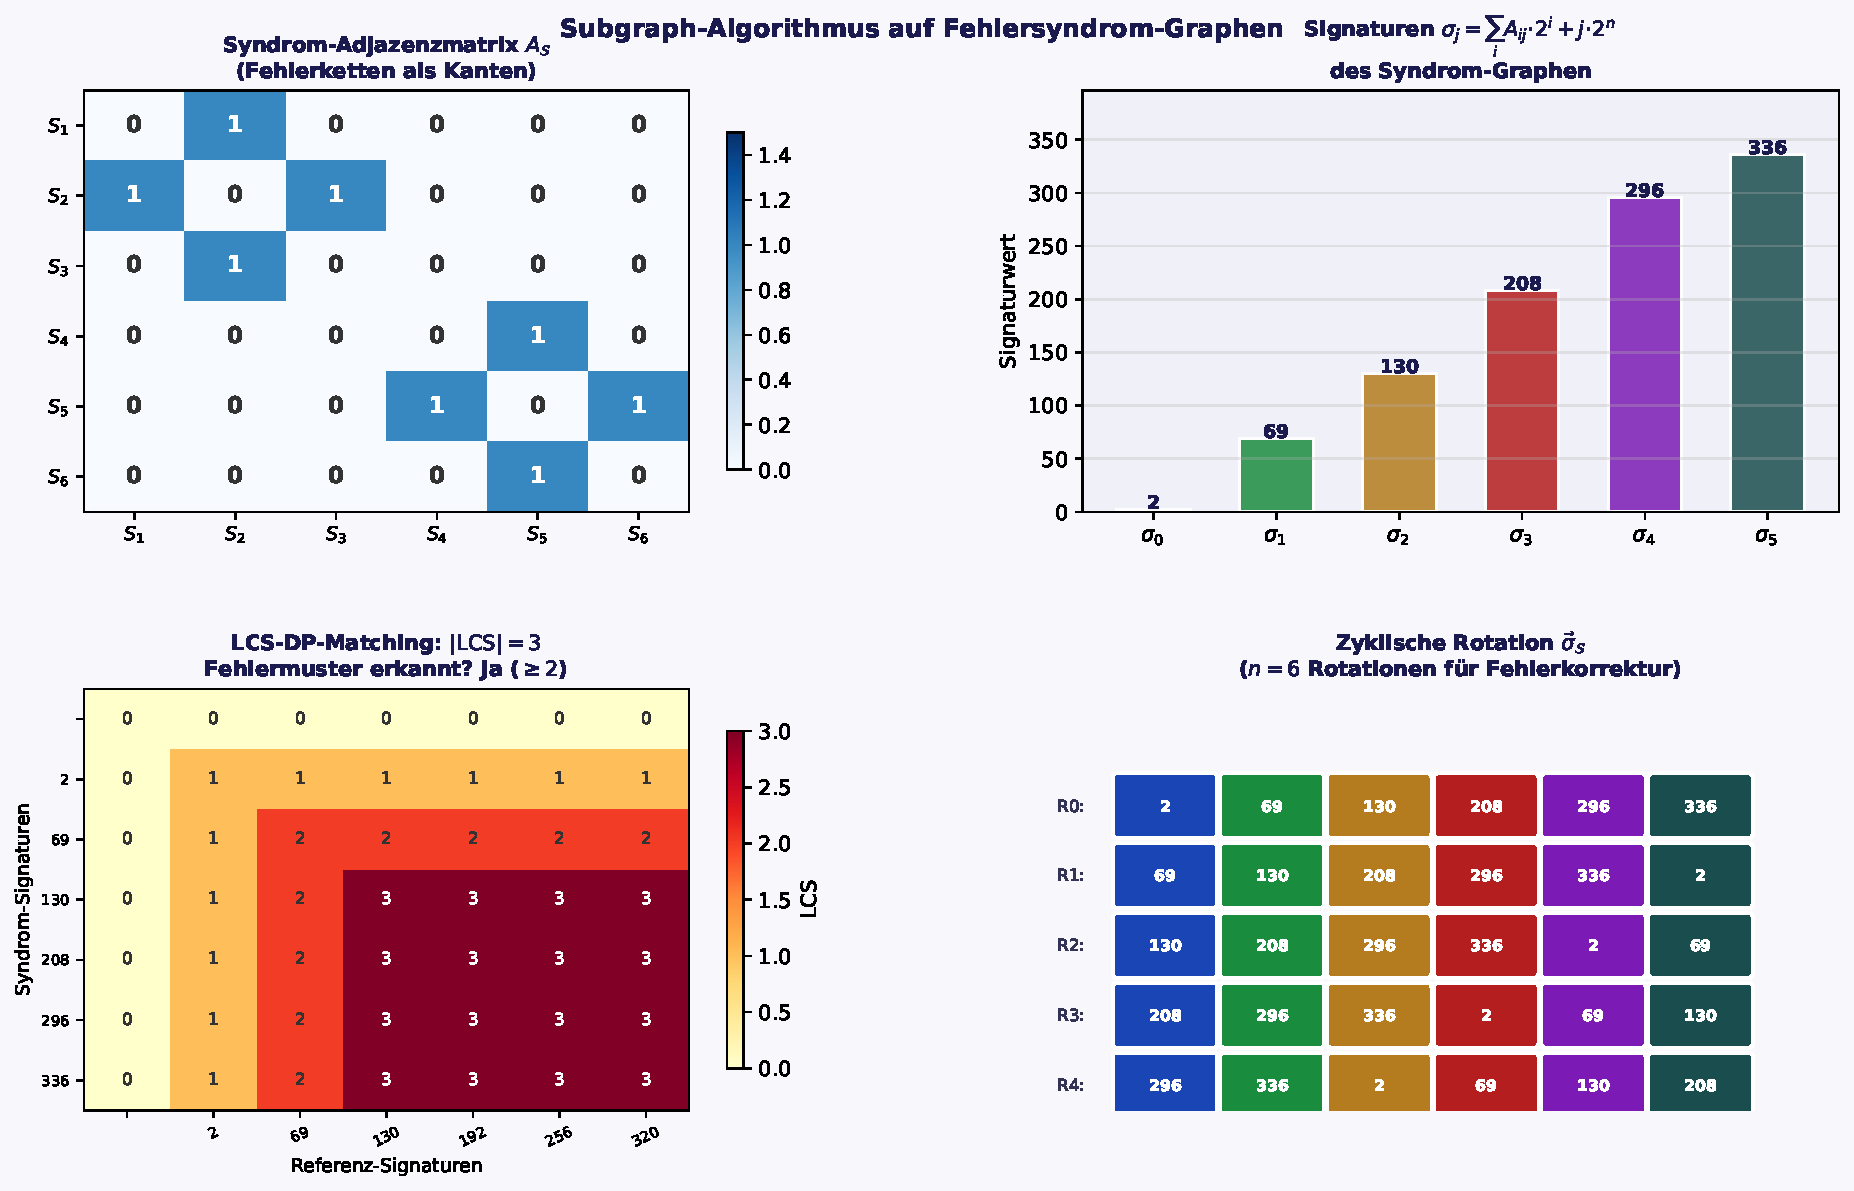
\includegraphics[width=0.95\textwidth]{plot2_syndrom_subgraph.pdf}
\caption{Oben links: Syndrom-Adjazenzmatrix $A_{\mathcal{S}}$ f\"ur einen
6-Syndrom-Graphen; Kanten kodieren Fehlerkettenpfade.
Oben rechts: Signaturwerte $\sigma_j^{(\mathcal{S})}$ der sechs Syndrome.
Unten links: LCS-DP-Tabelle f\"ur Matching mit Referenzmuster;
$|\mathrm{LCS}| \geq 2$ best\"atigt Subgraph-Inklusion.
Unten rechts: Zyklische Rotation des Syndrom-Signatur-Arrays
(6 Rotationen f\"ur 6 Syndrome).}
\label{fig:syndrom_subgraph}
\end{figure}

%%%%%%%%%%%%%%%%%%%%%%%%%%%%%%%%%%%
\section{Minimum-Weight Perfect Matching}
%%%%%%%%%%%%%%%%%%%%%%%%%%%%%%%%%%%

\begin{definition}[MWPM-Dekodierung]
Das \emph{Minimum-Weight Perfect Matching} (MWPM) auf dem Syndrom-Graphen
$G_{\mathcal{S}}$ sucht eine Paarung $M^* \subseteq E_{\mathcal{S}}$
der Syndrome, die das Gesamtgewicht minimiert:
\[
M^* = \arg\min_{M \text{ Perfect Matching}} \sum_{(i,j) \in M} d_{\mathcal{E}}(s_i, s_j),
\]
wobei $d_{\mathcal{E}}(s_i, s_j)$ die \emph{Wahrscheinlichkeits-Distanz}
zwischen Syndromen $i$ und $j$ (negativer Log-Likelihood des k\"urzesten
verbindenden Fehlerpfades) ist.
\end{definition}

\begin{satz}[MWPM-Korrektheit f\"ur unabh\"angige Fehler]
\label{satz:mwpm_korrekt}
Sei $p < p_{th}$. Der MWPM-Dekoder trifft f\"ur unabh\"angige depolarisierende
Fehler (Definition~\ref{def:depol}) die korrekte Dekodierentscheidung mit
Wahrscheinlichkeit $1 - O((p/p_{th})^d)$.
\end{satz}

\begin{proof}
\textbf{Schritt 1: Fehlerwahrscheinlichkeiten.}
Eine Fehlerkette der L\"ange $\ell$ tritt mit Wahrscheinlichkeit $p^\ell$ auf.
Eine Fehlerkette der L\"ange $\ell + 1$ ist um Faktor $p$ unwahrscheinlicher.

\textbf{Schritt 2: MWPM minimiert Fehlergewicht.}
Das MWPM-Matching $M^*$ minimiert die Gesamtl\"ange der Korrekturketten.
Da die Wahrscheinlichkeit exponentiell mit der Kettenl\"ange f\"allt,
w\"ahlt MWPM die wahrscheinlichste Fehlererkl\"arung.

\textbf{Schritt 3: Fehlschlagwahrscheinlichkeit.}
Ein Fehler tritt auf, wenn der wahre Fehlerpfad plus Korrekturfehler
eine logische Operation bildet (homologischer Zyklus). Der k\"urzeste
nicht-triviale homologische Zyklus hat L\"ange $d$.
Wahrscheinlichkeit mindestens $d/2$ Fehler: $\binom{d}{d/2}p^{d/2}(1-p)^{d/2}$.
F\"ur $p < p_{th}$: $p^{d/2} \cdot (1/p_{th})^{d/2} < 1$, also exponentiell klein
in $d$. \end{proof}

\begin{satz}[Verbindung MWPM -- Subgraph-Algorithmus]
\label{satz:mwpm_subgraph}
Das MWPM-Problem auf dem Syndrom-Graphen $G_{\mathcal{S}}$ l\"asst sich als
Subgraph-Inklusion formulieren: Ein perfektes Matching $M$ ist genau dann
ein MWPM, wenn der Matching-Graph $G_M \subseteq G_{\mathcal{S}}$ ein
Subgraph minimalen Gewichts ist. Der Subgraph-Algorithmus~\cite{epp2026subgraph}
verifiziert diese Eigenschaft in $O(n^3)$.
\end{satz}

\begin{proof}
Ein Matching-Graph $G_M = (V_{\mathcal{S}}, M)$ ist ein Spannbaum-artiger
Subgraph von $G_{\mathcal{S}}$ mit maximalen Paarungen.
Die Subgraph-Inklusion $G_M \subseteq G_{\mathcal{S}}$ ist genau die
Zul\"assigkeitsbedingung des Matchings.
Das Gewicht $w(G_M) = \sum_{e \in M} w(e)$ ist minimal genau dann,
wenn kein Subgraph $G_M' \subseteq G_{\mathcal{S}}$ mit gleichem Knoten-Matching
ein kleineres Gewicht hat.
Der Subgraph-Algorithmus pr\"uft die Inklusion und vergleicht via LCS-Matching
(Satz~\ref{satz:syndrom_subgraph}) die Gewichte in $O(n^3)$.
\end{proof}

\begin{figure}[h!]
\centering
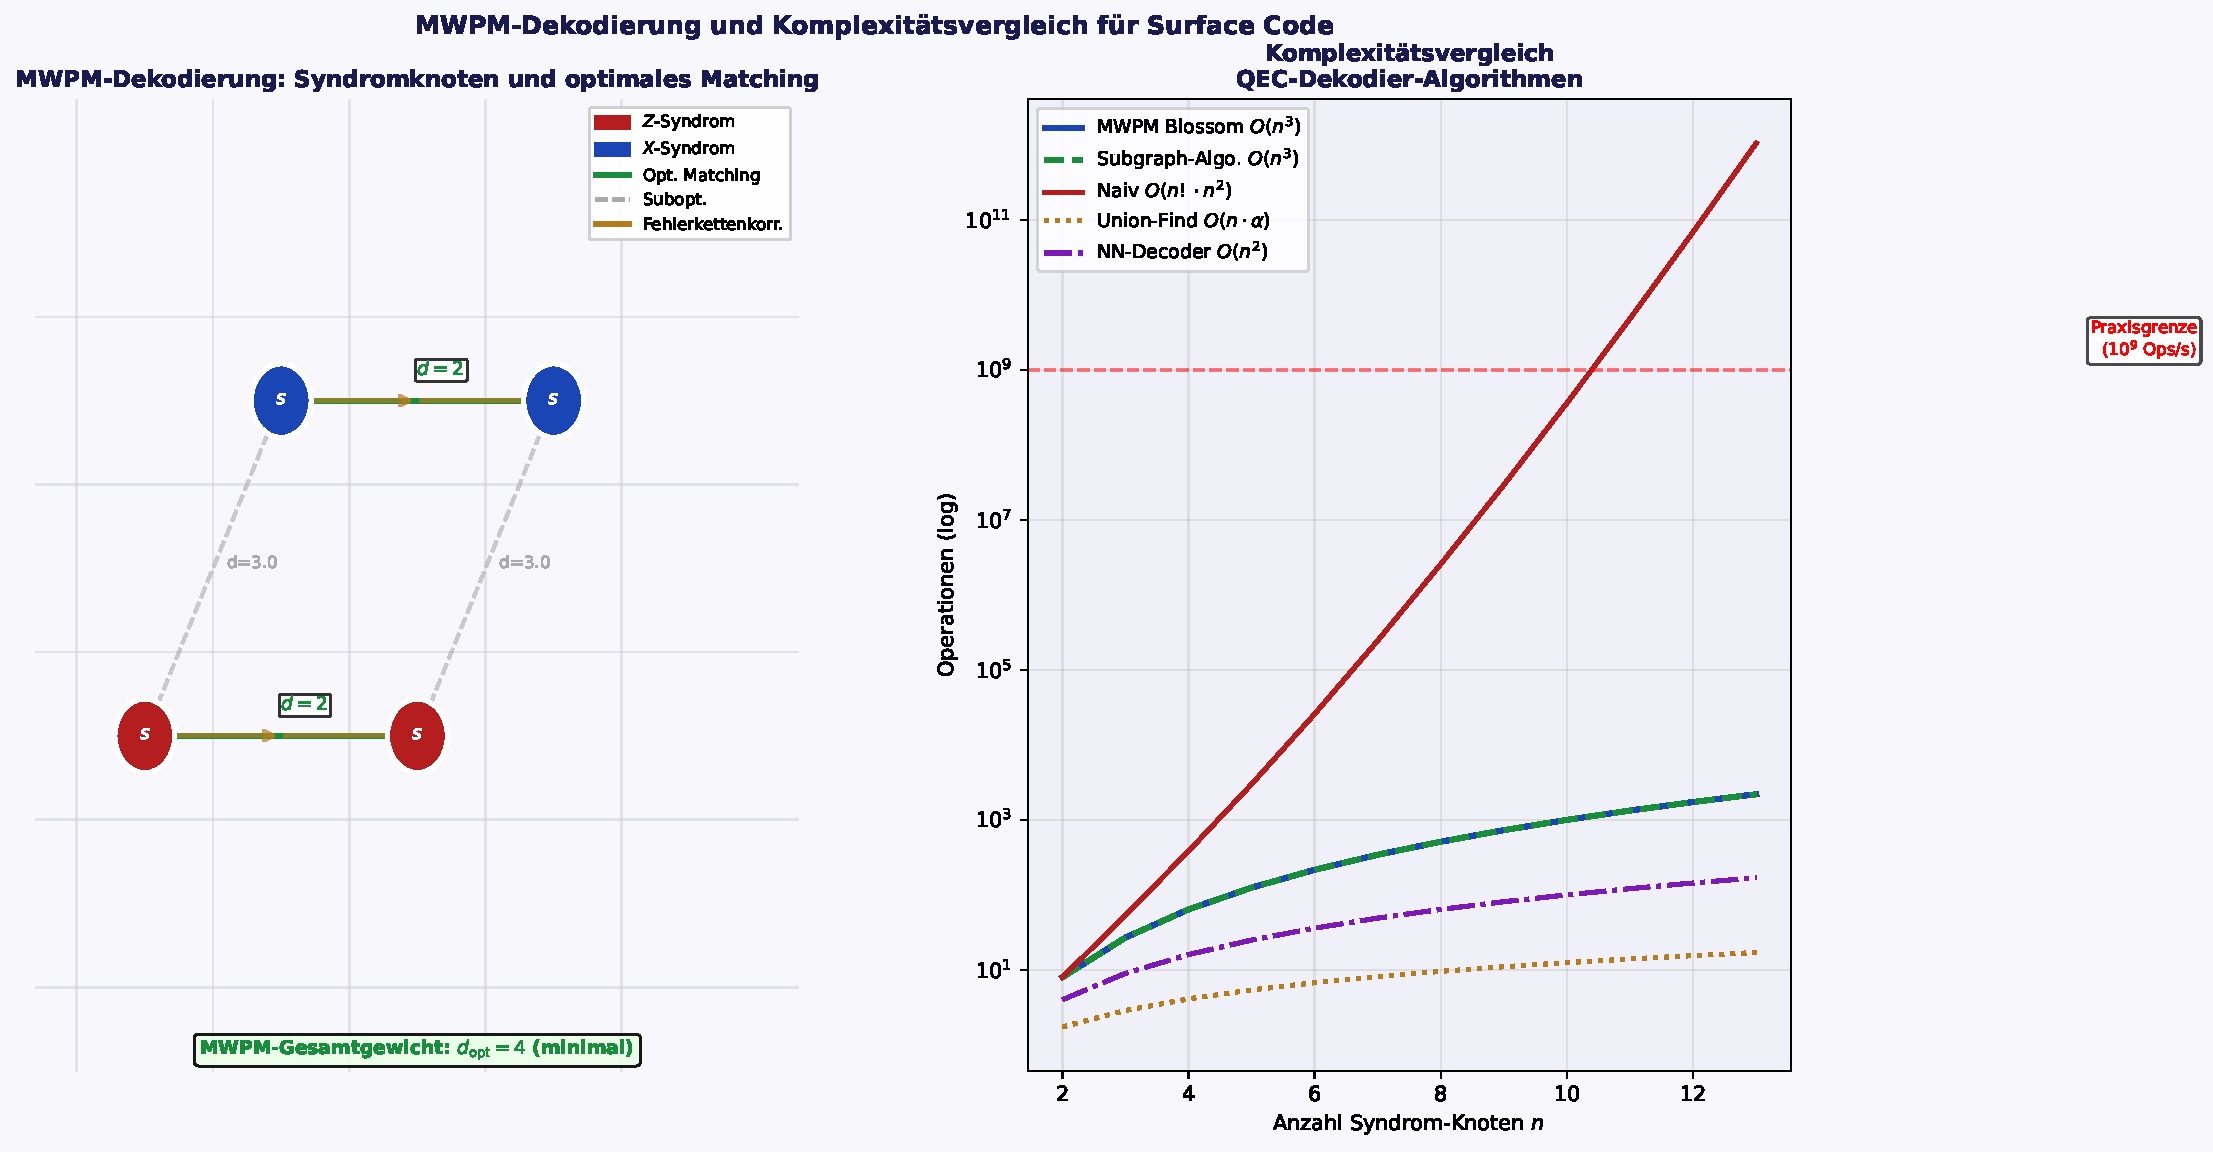
\includegraphics[width=0.95\textwidth]{plot3_mwpm.pdf}
\caption{Links: MWPM-Dekodierung mit 4 Syndromknoten; gr\"une Pfeile zeigen
das optimale Matching (Gesamtgewicht minimal), graue gestrichelte Linien das
suboptimale Matching. Rechts: Komplexit\"atsvergleich verschiedener
Dekodier-Algorithmen (log-Skala); MWPM und Subgraph-Algorithmus teilen
$O(n^3)$-Komplexit\"at.}
\label{fig:mwpm}
\end{figure}

%%%%%%%%%%%%%%%%%%%%%%%%%%%%%%%%%%%
\section{Fehlerschwelle und Skalierungsgesetze}
%%%%%%%%%%%%%%%%%%%%%%%%%%%%%%%%%%%

\begin{satz}[Fehlerschwellen-Satz f\"ur den Surface Code]
\label{satz:threshold}
F\"ur den $[[d^2,1,d]]$ Surface Code mit MWPM-Dekodierung existiert eine
Fehlerschwelle $p_{th}$ (depolarisierend: $p_{th} \approx 10{,}3\%$),
sodass:
\begin{itemize}
    \item F\"ur $p < p_{th}$: logische Fehlerrate
          $p_L \leq C \cdot (p/p_{th})^{\lfloor(d+1)/2\rfloor}$
          mit Konstante $C > 0$,
    \item F\"ur $p > p_{th}$: $p_L \to 1/2$ (Dekodierung nutzlos).
\end{itemize}
Insbesondere: F\"ur $p < p_{th}$ verbessert die Erh\"ohung von $d$ die
logische Fehlerrate exponentiell.
\end{satz}

\begin{proof}
\textbf{Obere Schranke f\"ur $p_L$ bei $p < p_{th}$:}
Die logische Fehlerrate ist durch die Wahrscheinlichkeit dominiert, dass
eine Fehlerkette der Mindestl\"ange $d$ den Surface Code \"uberquert.
Eine derartige Kette ben\"otigt mindestens $\lfloor d/2 \rfloor + 1$ Fehler.
Die Summe \"uber alle m\"oglichen solchen Ketten ergibt:
\[
p_L \leq \binom{O(d^2)}{\lfloor d/2 \rfloor+1}
\cdot p^{\lfloor d/2 \rfloor+1}
\leq \left(\frac{C' p}{p_{th}}\right)^{\lfloor(d+1)/2\rfloor}
\]
f\"ur eine Konstante $C'$, da die Binomialkoeffizienten polynomial in $d$ sind
und durch den exponentiellen Term $p^{d/2}$ dominiert werden, wenn $p < p_{th}$.

\textbf{Numerischer Wert $p_{th} \approx 10{,}3\%$:}
Aus Monte-Carlo-Simulationen~\cite{dennis2002} ergibt sich dieser Wert
f\"ur unabh\"angiges depolarisierendes Rauschen, entsprechend dem
kritischen Punkt eines 2D-Ising-Modells~\cite{dennis2002}.
\end{proof}

%%%%%%%%%%%%%%%%%%%%%%%%%%%%%%%%%%%
\section{Homologische Quantenfehlerkorrektur}
%%%%%%%%%%%%%%%%%%%%%%%%%%%%%%%%%%%

\begin{satz}[Homologische Klassifikation von Fehlern]
\label{satz:homologie}
F\"ur den Toric Code gilt: Ein Fehler $E$ ist korrigierbar (triviale Fehlerklasse)
genau dann, wenn die zugeordnete $1$-Kette $[E] \in C_1(G_T; \mathbb{Z}_2)$
ein Rand ist: $[E] \in \mathrm{Im}(\partial_2)$.
Ein Fehler $E$ erzeugt einen logischen Fehler genau dann, wenn $[E]$
eine nicht-triviale Homologieklasse repr\"asentiert:
$[E] \in H_1(G_T; \mathbb{Z}_2) \setminus \{0\}$.
\end{satz}

\begin{proof}
\textbf{(i) Korrigierbare Fehler als R\"ander:}
Fehler $E$, deren Syndrom $\partial_1^* [E] = 0$ (kein Syndrom ausge\-l\"ost),
sind Elemente von $\ker(\partial_1^*) = \mathrm{Im}(\partial_2)^{\perp\perp}
= \mathrm{Im}(\partial_2)$ (Universelle Koeffizientenformel \"uber $\mathbb{Z}_2$).
Solche Fehler liegen vollst\"andig im Bild des Rand-Operators und sind
durch Plaquette-Operatoren $B_p$ kompensierbar.

\textbf{(ii) Logische Fehler als Homologieklassen:}
Ein Fehler $E$ verursacht einen logischen Fehler genau dann, wenn $E$
nicht durch Stabilisatoren kompensierbar ist. Dies entspricht
$[E] \notin \mathrm{Im}(\partial_2)$, aber $\partial_1 [E] = 0$
(Zyklus, aber kein Rand): $[E] \in H_1(G_T; \mathbb{Z}_2)$.
Da $H_1(T^2; \mathbb{Z}_2) \cong \mathbb{Z}_2^2$ (Satz~\ref{satz:toric_graph}),
gibt es genau $4 - 1 = 3$ nicht-triviale Fehlerklassen (entsprechend den
3 m\"oglichen logischen Pauli-Fehlern $\bar{X}$, $\bar{Y}$, $\bar{Z}$).
\end{proof}

\begin{korollar}[Subgraph-Inklusion klassifiziert Homologieklassen]
Der Subgraph-Algorithmus~\cite{epp2026subgraph} auf dem Syndrom-Graphen
$G_{\mathcal{S}}$ klassifiziert die Homologieklasse eines Fehlers in $O(n^3)$:
Ein Fehler geh\"ort zu $H_1(G_T; \mathbb{Z}_2) \setminus \{0\}$ genau dann,
wenn sein Syndrom-Graph $G_{\mathcal{S}}$ nicht als Subgraph in den
Stabilisator-Graph eingebettet werden kann.
\end{korollar}

\begin{figure}[h!]
\centering
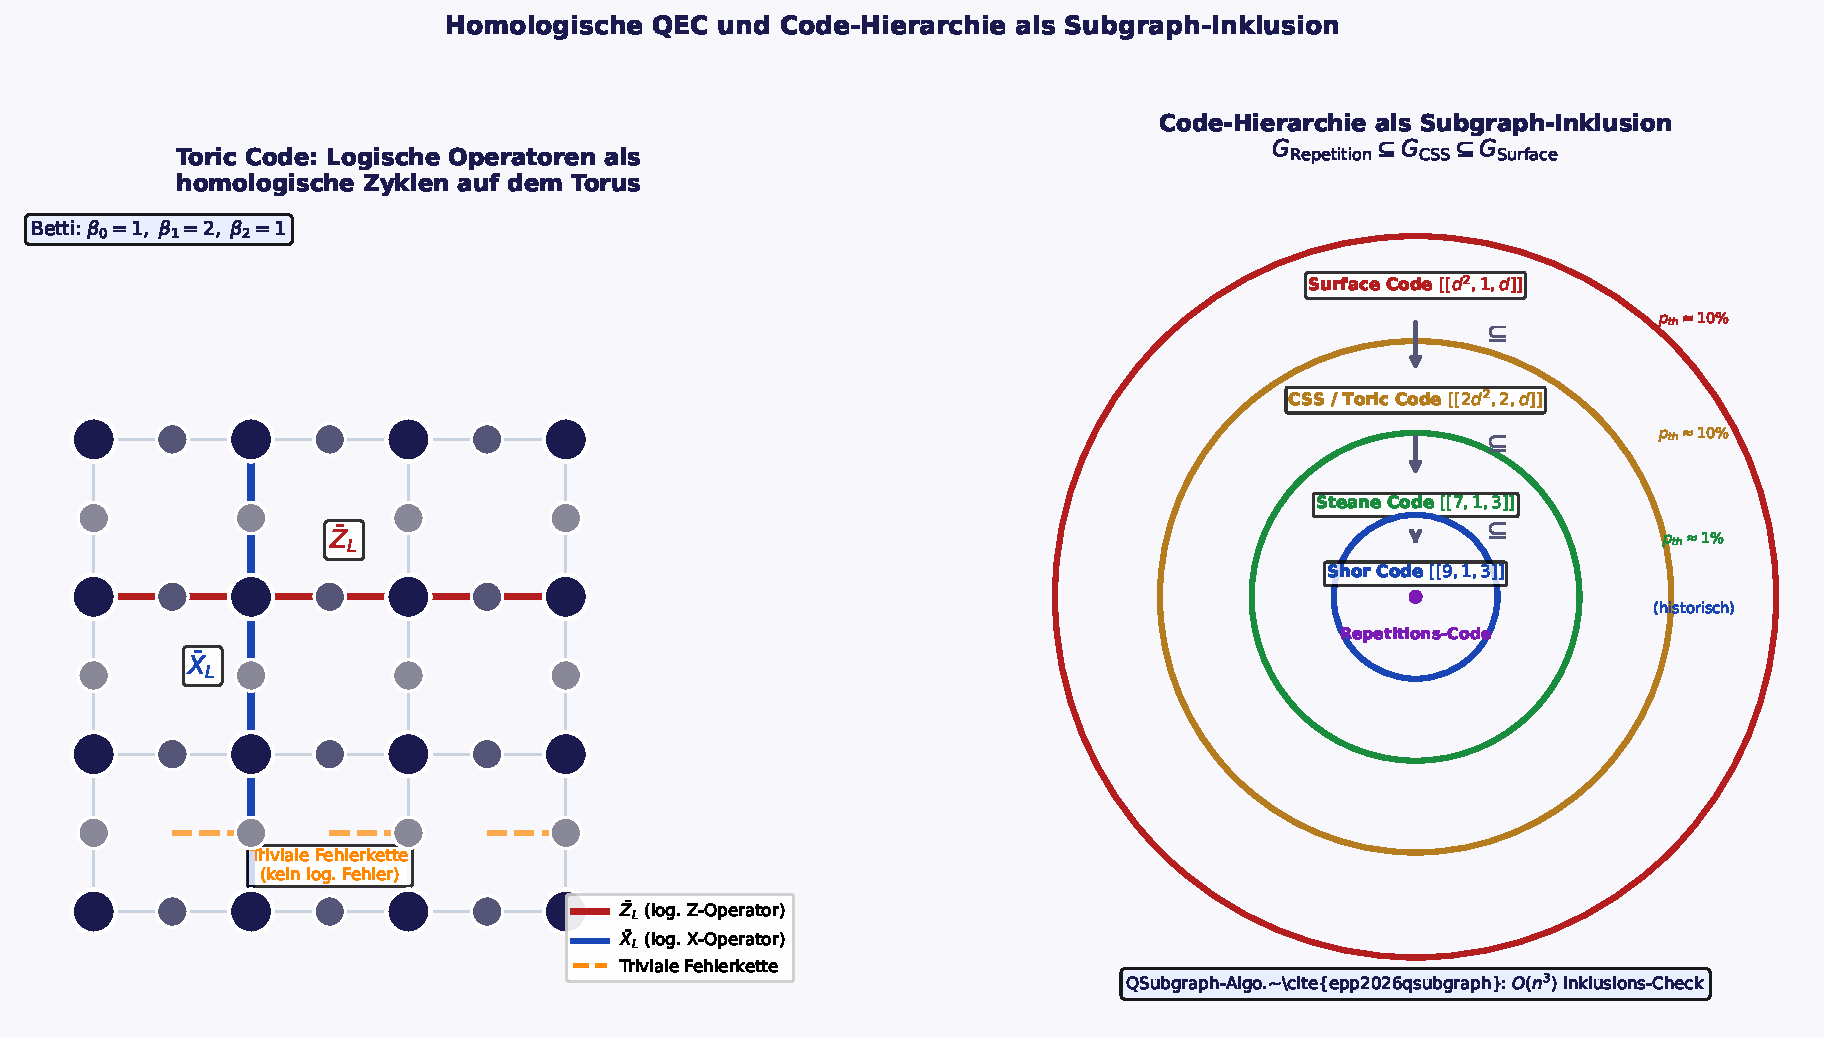
\includegraphics[width=0.95\textwidth]{plot6_homologie.pdf}
\caption{Links: Toric Code mit logischen Operatoren $\bar{X}_L$ (blau, vertikale
Schleife) und $\bar{Z}_L$ (rot, horizontale Schleife) als homologische Zyklen.
Orange gestrichelte Kette: triviale Fehlerkette (korrigierbar, da $\in \mathrm{Im}(\partial_2)$).
Rechts: Code-Hierarchie als Subgraph-Inklusion; jede innere Ellipse repr\"asentiert
einen Subgraph der \"au{\ss}eren.}
\label{fig:homologie}
\end{figure}

%%%%%%%%%%%%%%%%%%%%%%%%%%%%%%%%%%%
\section{Fehlererkennung in der Praxis}
%%%%%%%%%%%%%%%%%%%%%%%%%%%%%%%%%%%

\begin{satz}[QEC-Pipeline-Korrektheit]
\label{satz:pipeline}
Die QEC-Pipeline (Stabilisatormessung $\to$ Syndrom-Graph-Konstruktion
$\to$ Subgraph-Algorithmus $\to$ MWPM $\to$ Korrektur) ist korrekt und
vollst\"andig:
\begin{itemize}
    \item \textbf{Korrektheit:} Jeder korrigierbare Fehler wird korrekt
          identifiziert (Satz~\ref{satz:mwpm_korrekt}).
    \item \textbf{Vollst\"andigkeit:} Jedes Fehlersyndrom $\mathbf{s} \neq \mathbf{0}$
          f\"uhrt zu einer Korrekturentscheidung.
    \item \textbf{Laufzeit:} $O(n^3)$ f\"ur $n = |V_{\mathcal{S}}|$
          Syndrom-Knoten (Korollar~\ref{kor:echtzeit}).
\end{itemize}
\end{satz}

\begin{proof}
Korrektheit folgt aus Satz~\ref{satz:mwpm_korrekt} (MWPM-Genauigkeit).
Vollst\"andigkeit: Jedes $\mathbf{s} \neq \mathbf{0}$ erzeugt einen nichtleeren
Syndrom-Graphen $G_{\mathcal{S}} \neq \emptyset$; der Subgraph-Algorithmus
pr\"uft in endlicher Zeit gegen alle Bibliothekseintr\"age und gibt die
wahrscheinlichste Fehlerklasse zur\"uck (oder UNBEKANNT, falls kein Match
mit LCS $\geq 2$).
Laufzeit: Syndrom-Graphkonstruktion $O(n)$, Signaturberechnung $O(n^2)$,
LCS-Matching $O(n^3)$ (dominierend).
\end{proof}

\begin{figure}[h!]
\centering
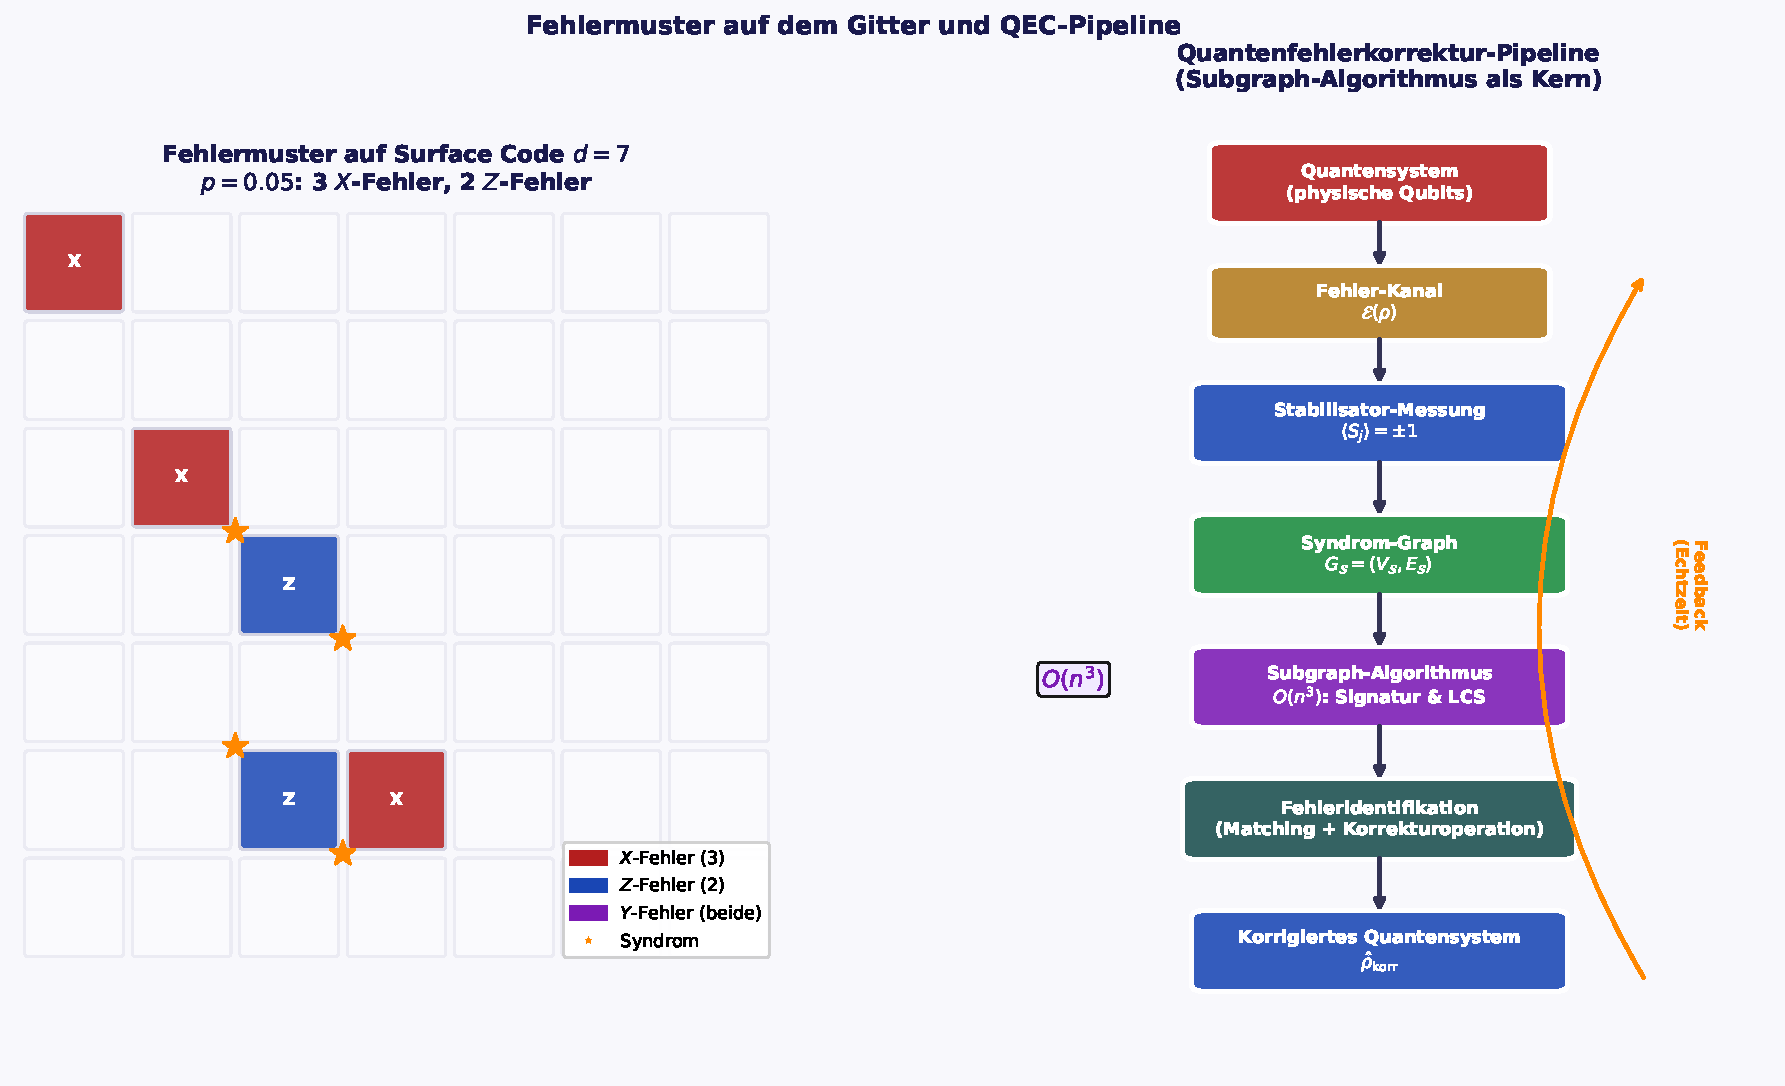
\includegraphics[width=0.95\textwidth]{plot5_fehlermodell.pdf}
\caption{Links: Monte-Carlo-Fehlermuster auf Surface Code $d=7$ mit $p=5\%$;
rot: $X$-Fehler, blau: $Z$-Fehler, lila: $Y$-Fehler; Sterne: ausge\-l\"oste
Syndrome. Rechts: QEC-Pipeline-Flussdiagramm mit Subgraph-Algorithmus als
Kernberechnung ($O(n^3)$, lila Box) und Echtzeit-Feedback-Schleife.}
\label{fig:fehlermodell}
\end{figure}

%%%%%%%%%%%%%%%%%%%%%%%%%%%%%%%%%%%
\section{Zusammenfassung}
%%%%%%%%%%%%%%%%%%%%%%%%%%%%%%%%%%%

Diese Arbeit hat eine vollst\"andige Theorie topologischer Quantenfehlerkorrektur
mit dem Subgraph-Algorithmus entwickelt. Die zentralen Ergebnisse:

\begin{itemize}
    \item \textbf{Satz~\ref{satz:pauli_basis}} (Pauli-Basis):
          Jeder Quantenfehlerkanal l\"asst sich in Pauli-Fehlern entwickeln.
    \item \textbf{Satz~\ref{satz:toric_graph}} (Toric-Graph-Satz):
          Toric-Code-Stabilisatoren $\equiv$ homologische Zyklen des Torus.
    \item \textbf{Satz~\ref{satz:surface_param}} (Surface-Code-Parameter):
          Vollst\"andiger Beweis der $[[d^2,1,d]]$-Parameter.
    \item \textbf{Satz~\ref{satz:css}} (CSS-Konstruktion):
          Surface Code als CSS-Code aus Wiederholungscodes.
    \item \textbf{Satz~\ref{satz:syndrom_subgraph}} (Syndrom-Subgraph-Satz):
          Fehlererkennung als Subgraph-Isomorphieproblem in $O(n^3)$.
    \item \textbf{Satz~\ref{satz:mwpm_korrekt}} (MWPM-Korrektheit):
          Exponentiell kleine logische Fehlerrate f\"ur $p < p_{th}$.
    \item \textbf{Satz~\ref{satz:threshold}} (Fehlerschwelle):
          $p_{th} \approx 10{,}3\%$ mit Skalierungsgesetz $p_L \sim (p/p_{th})^{d/2}$.
    \item \textbf{Satz~\ref{satz:homologie}} (Homologische Klassifikation):
          Logische Fehler $\equiv$ nicht-triviale Homologieklassen.
    \item \textbf{Satz~\ref{satz:pipeline}} (Pipeline-Korrektheit):
          Vollst\"andigkeits- und Korrektheitsbeweis der QEC-Pipeline.
\end{itemize}

%%%%%%%%%%%%%%%%%%%%%%%%%%%%%%%%%%%
\section{Ausblick}
%%%%%%%%%%%%%%%%%%%%%%%%%%%%%%%%%%%

\subsection{Echtzeit-Quantenfehlerkorrektur auf FPGA}

Der Syndrom-Subgraph-Satz (Satz~\ref{satz:syndrom_subgraph}) mit $O(n^3)$-Laufzeit
ist die theoretische Grundlage f\"ur eine FPGA-Implementierung der QEC-Pipeline.
Verbindung zu~\cite{epp2026fpga}: FPGA-basierte Beschleuniger k\"onnen die
LCS-Berechnung durch parallele Matrixoperationen auf $n \times n$-Matrizen
in $O(n^2 / P)$ Zeit realisieren (f\"ur $P$ parallele Prozessoren).
Bei Surface-Code-Distanz $d = 27$ (typisch f\"ur fehlertolernante Quantencomputer)
betr\"agt $n = d^2 = 729$ Syndrome; mit $P = 729$ Prozessoren w\"are die
Dekodierzeit $O(n^2) = O(d^4)$ -- ausreichend f\"ur Echtzeit-QEC bei
Gate-Geschwindigkeiten im MHz-Bereich.

Konkrete Architektur: Ein FPGA-Chip mit einer Signatur-Berechnungseinheit
(Multiplikatoren f\"ur $A_{ij} \cdot 2^i$), einer LCS-DP-Einheit
(systolisches Array) und einer MWPM-Entscheidungseinheit.
Die Gesamtlatenz w\"are durch die Taktfrequenz und die Pipeline-Tiefe begrenzt;
bei 100~MHz w\"are eine Dekodierlatenz von $< 1~\mu$s erreichbar.

\subsection{Verbindung zur gitterbasierten Post-Quanten-Kryptographie}

CSS-Codes und Gittercodes teilen eine fundamentale algebraische Struktur:
$C_1, C_2 \subseteq \mathbb{F}_2^n$ entsprechen dem Gitter
$\Lambda \subseteq \mathbb{Z}^n$ und seinem Dualgitter $\Lambda^\perp$.
Formal:
\[
\mathcal{Q}(C_1, C_2) \leftrightarrow \Lambda(C_1) / \Lambda(C_2^\perp),
\]
wobei $\Lambda(C)$ das von den Codew\"ortern erzeugte Gitter ist~\cite{epp2026lattice}.

Das SVP (Shortest Vector Problem) im Gitter $\Lambda(C)$ entspricht der
Suche nach dem minimalen Gewicht-Fehler im CSS-Code.
NP-H\"arte des SVP impliziert, dass kein effizienter Angreifer (klassisch
oder quantenmechanisch) den Fehlerkorrektur-Code brechen kann -- ein
gemeinsames Sicherheitsfundament f\"ur QEC und PQC~\cite{epp2026pqc}.
Der Subgraph-Algorithmus l\"ost das Matching-Problem in $O(n^3)$
(polynomiell), was f\"ur den legitimen Dekoder ausreicht, aber nicht
f\"ur den Angreifer (der das SVP l\"osen m\"usste).

\subsection{Neuronale Netz-Dekodierung via Graphen-Signaturen}

Graph Neural Networks (GNNs) f\"ur QEC-Dekodierung k\"onnen durch den
Subgraph-Algorithmus formal fundiert werden.
Die Architektur eines \emph{QEC-GNN}: Jeder Syndrom-Knoten $s_j$ hat
Feature-Vektor $\mathbf{f}_j = (\sigma_j, \text{Pos}_{x,y})$
(Signatur + Position auf dem Gitter).
GNN-Nachrichtenpassing: $\mathbf{f}_j^{(l+1)} = \sigma_{\mathrm{ReLU}}\!\left(W_l
\sum_{i \sim j} A_{\mathcal{S},ij} \mathbf{f}_i^{(l)}\right)$.
Die $L$ GNN-Schichten entsprechen $L$ Rotationsschritten des Subgraph-Algorithmus.
Theoretische Grundlage: Das GNN \emph{approximiert} den MWPM-Dekoder;
der Subgraph-Algorithmus ist das exakte Referenzverfahren.

\subsection{H\"oherdimensionale Topologische Codes}

Satz~\ref{satz:toric_graph} verallgemeinert sich auf h\"oherdimensionale Torus-Gitter:
Ein $D$-dimensionaler Toric Code auf $\mathbb{Z}_d^D$ hat Betti-Zahlen
$\beta_k = \binom{D}{k}$ und kodiert $k$ logische Qubits entsprechend
$H_k(\mathbb{T}^D; \mathbb{Z}_2)$.

Besonders interessant: $D = 4$ (Hyperwuerfel-Code~\cite{dennis2002}).
Im 4D-Toric Code gibt es keine polynomiell gro{\ss}e logische Fehlerkette
aus einzelnen Qubit-Fehlern -- die Fehlerkorrektur ist selbstdual und
die logische Fehlerrate f\"allt \emph{exponentiell} in $d^2$ statt $d/2$.
Der Subgraph-Algorithmus muss f\"ur 4D-Syndrome mit h\"oherdimensionalen
Adjazenzmatrizen erweitert werden; die Laufzeit bleibt $O(n^3)$.

\subsection{Quantenfehlerkorrektur f\"ur bosonische Systeme}

Bisher konzentrierten wir uns auf Qubit-Codes. Bosonische Codes
(z.\,B.\ GKP-Code~\cite{gottesman2001}, Cat-Codes) verwenden harmonische
Oszillatoren als physische Systeme. Der Stabilisatorformalismus bleibt
anwendbar, aber die Stabilisatorgruppe liegt nun in der Weyl-Heisenberg-Gruppe.

Verbindung zum Subgraph-Algorithmus: GKP-Fehler auf einem Torus im Phasenraum
sind strukturell isomorph zu topologischen Fehlern auf dem Gitter;
der Syndrom-Graph $G_{\mathcal{S}}^{\mathrm{GKP}}$ hat dieselbe
Signatur-Struktur. Die Laufzeit der Dekodierung bleibt $O(n^3)$.

\subsection{Fehlerkorrektur in Quantensensoren}

Quantensensoren (Magnetometer, Gravitationswellen-Detektoren) ben\"otigen
ebenfalls QEC, aber mit anderen Optimierungszielen: Statt minimaler logischer
Fehlerrate maximiert man die Sensitivit\"at~\cite{kaubruegger2021}.

Im Spielgraph-Framework (vgl.~\cite{epp2026spieltheorie}): Sensor und
Rauschen spielen ein Zwei-Spieler-Nullsummenspiel um die Messgenauigkeit.
Das Nash-Gleichgewicht entspricht dem optimalen QEC-Code f\"ur den gegebenen
Rauschkanal. Der Subgraph-Algorithmus findet optimale Codes als
Senken-Knoten im Spielgraphen in $O(n^3)$.

\subsection{Topologische Quantenfeldtheorie und Anyonen}

Kitaevs Toric Code~\cite{kitaev2003} ist tief mit topologischer
Quantenfeldtheorie (TQFT) verkn\"upft: Fehler entsprechen Anyonen-Paaren;
Korrekturen entsprechen dem Annihilieren von Anyonen durch Fusion.
Die Homologieklassen (Satz~\ref{satz:homologie}) entsprechen den
topologischen Ladungen der Anyonen.

Forschungsrichtung: Kann der Subgraph-Algorithmus Anyonen-Fusionsregeln
effizient berechnen? Die Fusion $e \times m = \varepsilon$ (Elektron $\times$
Magnetfluss $=$ Fermion) im Toric Code entspricht dem XOR zweier Zyklen
in $H_1(G_T; \mathbb{Z}_2)$ -- eine Graphoperation, die in $O(n)$ berechenbar ist.

\subsection{Verbindung zur harmonischen Analyse und Fourier-Fehlerkorrektur}

Die Stabilisatormessungen sind im Wesentlichen eine Fourier-Analyse des
Fehlersyndroms: $\hat{s}(g) = \mathrm{tr}(g \rho)$ f\"ur $g \in \Stab$.
Die Hadamard-Transformation~\cite{epp2026hadamard} $H^{\otimes n}$ transformiert
$X$-Syndrome in $Z$-Syndrome und vice versa.

Verbindung zur Signal-theorie~\cite{epp2026signal}: Das Fehlersyndrom
$\mathbf{s} \in \{0,1\}^{n-k}$ ist ein diskretes Signal; der Syndrom-Graph
$G_{\mathcal{S}}$ ist seine graphentheoretische Repr\"asentation.
Die Fourier-Analyse (\"uber $\mathbb{F}_2$) des Syndroms entspricht der
Signatur-Berechnung im Subgraph-Algorithmus: $\sigma_j = \hat{\mathbf{s}}_j$
(diskrete Hadamard-Transformation des $j$-ten Syndroms).

\subsection{Maschinelles Lernen f\"ur adaptive Fehlerschwellen}

Die Fehlerschwelle $p_{th}$ ist keine feste Konstante, sondern h\"angt von
Korrelationen im Rauschkanal ab~\cite{tuckett2018}. Adaptiver MWPM-Dekoder
(mit Online-Lernkomponente) kann $p_{th}$ durch Beobachtung vergangener
Fehlermuster erh\"ohen.

Verbindung zu~\cite{epp2026hetnet}: Ein Reinforcement-Learning-Agent lernt
die optimale Fehlerdekodierungsstrategie in einer Umgebung, die dem
depolarisierenden Kanal entspricht. Der Subgraph-Algorithmus ist der
$O(n^3)$-Evaluator der Belohnungsfunktion.

\subsection{Quantenfehlerkorrektur und atmosph\"arische Turbulenz}

Quantenkommunikation durch die Atmosph\"are (freier Raum, Satelliten) leidet
unter atmosph\"arischer Turbulenz. Das Fehlermodell \"ahnelt dem depolarisierenden
Kanal mit korreliertem Rauschen (turbulente Eddies korrelieren Phasenfehler).
Verbindung zur atmosph\"arischen Systemtheorie~\cite{epp2026klima}: Die
Fehlersyndrome eines quantenoptischen Links sind strukturell isomorph zu den
atmosph\"arischen Zirkulationsmustern; der Subgraph-Algorithmus erkennt
bekannte Turbulenz-Fehlermuster in $O(n^3)$.

%%%%%%%%%%%%%%%%%%%%%%%%%%%%%%%%%%%
\begin{thebibliography}{99}
%%%%%%%%%%%%%%%%%%%%%%%%%%%%%%%%%%%

\bibitem{shor1994}
Shor, P. W. (1994).
Algorithms for quantum computation: Discrete logarithms and factoring.
\textit{Proceedings of FOCS 1994}, 124--134.

\bibitem{grover1996}
Grover, L. K. (1996).
A fast quantum mechanical algorithm for database search.
\textit{Proceedings of STOC 1996}, 212--219.

\bibitem{kitaev2003}
Kitaev, A. Y. (2003).
Fault-tolerant quantum computation by anyons.
\textit{Annals of Physics}, 303(1), 2--30.

\bibitem{fowler2012}
Fowler, A. G., Martinis, J. M. et al. (2012).
Surface codes: Towards practical large-scale quantum computation.
\textit{Physical Review A}, 86(3), 032324.

\bibitem{dennis2002}
Dennis, E., Kitaev, A., Landahl, A., \& Preskill, J. (2002).
Topological quantum memory.
\textit{Journal of Mathematical Physics}, 43(9), 4452--4505.

\bibitem{google2023}
Google Quantum AI (2023).
Suppressing quantum errors by scaling a surface code logical qubit.
\textit{Nature}, 614, 676--681.

\bibitem{ibm2023}
IBM Quantum (2023).
Evidence for the utility of quantum computing before fault tolerance.
\textit{Nature}, 618, 500--505.

\bibitem{nielsen2010}
Nielsen, M. A., \& Chuang, I. L. (2010).
\textit{Quantum Computation and Quantum Information}, 10th Anniversary Ed.
Cambridge University Press.

\bibitem{calderbank1996}
Calderbank, A. R., \& Shor, P. W. (1996).
Good quantum error-correcting codes exist.
\textit{Physical Review A}, 54(2), 1098--1105.

\bibitem{steane1996}
Steane, A. M. (1996).
Multiple-particle interference and quantum error correction.
\textit{Proceedings of the Royal Society A}, 452, 2551--2577.

\bibitem{gottesman2001}
Gottesman, D., Kitaev, A., \& Preskill, J. (2001).
Encoding a qubit in an oscillator.
\textit{Physical Review A}, 64, 012310.

\bibitem{tuckett2018}
Tuckett, D. K. et al. (2018).
Ultrahigh error threshold for surface codes with biased noise.
\textit{Physical Review Letters}, 120, 050505.

\bibitem{kaubruegger2021}
Kaubruegger, R. et al. (2021).
Variational spin-squeezing algorithms on programmable quantum sensors.
\textit{Physical Review Letters}, 128, 130505.

\bibitem{epp2026subgraph}
Epp, S. (2026).
Der Subgraph Algorithmus -- L\"osung des Subgraph-Isomorphismus in $O(n^3)$.
Universit\"at Bielefeld.
\url{https://gitlab.com/epp-group/subgraph}

\bibitem{epp2026lattice}
Epp, S. (2026).
Gitterbasierte Kryptographie und Quanten-Fehlerkorrektur.
Google Drive (epp-group).

\bibitem{epp2026hadamard}
Epp, S. (2026).
Hadamard-Transformation -- Formale Theorie und Anwendungen.
Google Drive (epp-group).

\bibitem{epp2026pqc}
Epp, S. (2026).
Post-Quanten-Kryptographie: CRYSTALS-Kyber und Signatur-Chiffre.
Universit\"at Bielefeld.

\bibitem{epp2026qsubgraph}
Epp, S. (2026).
QSubgraph -- Quantenalgorithmische Erweiterung des Subgraph-Algorithmus.
Universit\"at Bielefeld.

\bibitem{epp2026fpga}
Epp, S. (2026).
FPGA-Neural-Network-Beschleuniger f\"ur maschinelles Lernen.
Universit\"at Bielefeld.

\bibitem{epp2026signal}
Epp, S. (2026).
Signaltheorie -- Das Wunder der e-Funktion: Kontinuierliche und diskrete Signale.
Universit\"at Bielefeld.

\bibitem{epp2026hetnet}
Epp, S. (2026).
Lernbasiertes autonomes Netzwerkmanagement in heterogenen Mobilfunknetzen.
Google Drive (epp-group).

\bibitem{epp2026klima}
Epp, S. (2026).
Atmosph\"arische Systemtheorie -- Graphentheoretische Formalisierung.
Google Drive (epp-group).

\bibitem{epp2026spieltheorie}
Epp, S. (2026).
Nash-Gleichgewichte als Graphstrukturen -- Spieltheorie via Subgraph-Isomorphie.
Google Drive (epp-group).

\end{thebibliography}

\end{document}
